\documentclass[a4paper,12pt,numbers=enddot]{scrreprt}	% numbers=enddot fa seguire il puntino dopo il numero di cap. noenddot lo toglie 
\usepackage[utf8]{inputenc}	%imposta la codifica di input; invece di "latin1", anche "utf8" va bene
\usepackage[footnotesize,it]{caption}	%per i cara piccoli
\usepackage[english]{babel}	%l?ultima lingua � quella predefinita
\usepackage{listings}		%codice sorgente
\lstset{frame=shadowbox, rulesepcolor=\color{blue}, breaklines=true, basicstyle=\small\ttfamily, columns=fullflexible,  keepspaces=true}	%disegna un rettangolo attorno al codice sorgente
\usepackage{indentfirst}	%rientra il primo paragrafo di ogni sezione
\usepackage{amsmath}%,amssymb,amsthm       % indispensabili per la matematica
\usepackage{graphicx}		% per inserire le immagini
\usepackage{graphics}		%?
\usepackage{sidecap}		%per mettere caption a lato della figuta
 % didascalie personalizzate
\usepackage{caption}		
\usepackage[numbers]{natbib} %?
\usepackage{psfrag} %?
\usepackage{multirow}	%?
\usepackage{booktabs} 	%?
\usepackage{lscape}%?
\usepackage{longtable}%?  %%
\usepackage{enumitem}%?
\usepackage{epsfig}		%per mettere fig usando comando tabular
\usepackage{makeidx}	%indice
\usepackage{varioref}
\usepackage[table]{xcolor}
\usepackage{epstopdf}
\usepackage{wrapfig}
%Setta dimensioni body
\usepackage[total={16.5cm,25cm},
						top=3.5cm,
						bottom=3.5cm,
						left=2.5cm,
						right=2.5cm,
						%includefoot,
						centering]{geometry}

\usepackage{wallpaper}%?
\usepackage{color}%?
\usepackage{setspace}		%per definire con dopo l'interlinea con \onehalfspacing
\onehalfspacing
\usepackage{appendix}
\usepackage{acronym}%?
\usepackage{makecell}
\usepackage{todonotes} %%todo things
%\usepackage{textgreek} %% per lettere greche nel testo
\usepackage{verbatim}


%Intestazioni e pie? pag.  
\usepackage[automark,headsepline,footsepline,autooneside,plainheadsepline,plainfootsepline]{scrpage2}	%i comandi plain-ecccc servono a dire che nella prima pag. del nuovo cap. voglio queste cose.
\usepackage[pagebackref=true, colorlinks=true, linkcolor=blue, hyperindex=true, urlcolor=blue, citecolor = green, linktocpage=true]{hyperref}		% indici e riferimenti cliccabili
\pagestyle{scrheadings}
\clearscrheadfoot
\ihead [Francesco Bonfadelli]{Francesco Bonfadelli}	%Kopfzeile Innen
\chead {}					%Kopfzeile Mitte
\ohead [\headmark]{\headmark}			%Kopfzeile Au�en
\ifoot {}					%Fu�zeile Innen
\cfoot[\pagemark]{\pagemark} 			%Fu�zeile Mitte
\ofoot {}

\automark[chapter]{chapter}
\KOMAoptions{cleardoublepage=scrheadings}	%per lasciate style=scrheadings anche per le pag vuoto (svuotate col comando cleardoublepage), si puo? anche scegliere cleardoublepage=plain o empty

\footskip=30pt	 %	abbassa il margine inf della pag
\setlength{\headheight}{2\baselineskip}

\newcommand\SectionFontStyle{\rmfamily}			% geh�rt zu den beiden folgenden setkomafont , keine ahnung was es macht =)
\setkomafont{chapter}{\huge\bfseries\SectionFontStyle}	% Chapter in der gleichen schriftart SectionFontStyle
\setkomafont{sectioning}{\bfseries\SectionFontStyle}
%Crea i link nel pdf (vedere come si fa a farli verdino e con i collegamenti solo sui numeri, non questi rettangoli cessi rossi	


\makeindex
\begin{document}

\renewcommand{\bibname}{References}	%to change the name: bibliography to references




%\pagenumbering{roman}
%\pagestyle{plain}
%******************************************************************
% Materiale iniziale
%******************************************************************
\begin{otherlanguage*}{italian} % da commentare se non si scrive in italiano



	\begin{titlepage}   %Frontespizio
\begin{center}
{\large UNIVERSIT\`A DEGLI STUDI DI BRESCIA}

\vspace{0.2cm}

{\large FACOLT\`A DI INGEGNERIA}
\vspace{0.2cm}

\begin{figure*}[htbp] 
\begin{center}
 \begin{tabular}{c c}
\raisebox{-.5\height}{
\includegraphics[width=0.40\textwidth]{images/00-loghi/logo_UniBS.eps}}
\end{tabular}
\end{center}
\end{figure*}

% \vspace{0.5cm}
{\large CORSO DI LAUREA MAGISTRALE IN INGEGNERIA INFORMATICA} \\


%\vspace{0.8cm}
\vspace{1.4cm}
{\huge \emph{\textbf{Accordatore digitale per chitarra}}} \\



\vspace{1.0cm}

{\Large{\emph{Elaborato di Digital Audio Processing}}} \\

\vspace{1.5cm}





\begin{flushright}
Studente: \\
\textbf{Francesco Bonfadelli} \\
\vspace{0.05cm}
\textbf{Matricola 83174} \\
\vspace{1.5cm}
\end{flushright}

\large{Anno Accademico 2011-2012}

\end{center}
\end{titlepage}


	\pagenumbering{roman}
	\tableofcontents

	\newpage
	%\thispagestyle{empty}
	%\mbox{}

	\pagenumbering{arabic}

	\chapter{Introduzione}

Per suonare musica di alta qualità, è necessario avere strumenti perfettamente accordati.
Come tutti i musicisti sanno, accordare uno strumento può essere difficoltoso, soprattutto per un orecchio non perfettamente allenato.
In questa relazione, si discute la realizzazione in Matlab di un software che rappresenta un accordatore digitale, cioè un programma che registra il suono prodotto dalla corda di una chitarra, lo analizza calcolando la frequenza fondamentale e rappresenta la differenza rispetto a una frequenza di riferimento, che è scelta tra le frequenze fondamentali delle corde dello strumento.
Questo lavoro rappresenta il progetto del corso di \emph{Digital Audio Processing} della Facoltà di Ingegneria dell'Università degli Studi di Brescia.

La nota prodotta da una corda della chitarra non è composta da una singola frequenza ma da un certo numero di armoniche. 
Il \emph{timbro}, cioè l'insieme delle armoniche prodotte da un determinato strumento, è ciò che distingue i diversi strumenti musicali tra loro quando suonano la stessa nota \cite{garzanti_timbro}.
Nel momento in cui una nota viene suonata, l'accordatore deve stabilire la frequenza fondamentale corrispondente.
Una delle parti principali di questo lavoro consiste proprio nel calcolo della frequenza fondamentale a partire dallo spettro del segnale della nota.

Un'altro argomento fondamentale trattato è il dimensionamento dei due parametri frequenza di campionamento e ampiezza del frame temporale registrato al fine di garantire il funzionamento in tempo reale del software mantenendo una precisione accettabile in frequenza.
Questi due requisiti richiedono valori di parametri in contrasto l'uno con l'altro.
Di seguito si discute ampiamente questo fatto e si propone una soluzione per aumentare la risoluzione ottenuta senza modificare i due valori scelti.

L'analisi del rumore in ingresso, prima operazione realizzata, e la realizzazione dell'interfaccia grafica del software, completano il lavoro svolto.

	\newpage
	\chapter{Analisi del Rumore In Ingresso}\label{cap:rumore}

Il primo passo per analizzare il segnale audio in ingresso è quello di valutare il rumore presente durante le operazioni di registrazione e conversione analogico-digitale del segnale effettuate dalla scheda audio. 

Per valutare tale fenomeno sono state realizzate diverse registrazioni in assenza di segnale utile. 
Per evitare che l'analisi del rumore venisse influenzata da effetti temporanei che concentrassero la maggior parte dell'energia in particolari frequenze, le misure sono state effettuate in diversi momenti della giornata.
Inoltre, dal momento che non si può escludere la presenza di disturbi esterni casuali concentrati in particolari frequenze, si è cercato di isolare il più possibile la zona di registrazione da tali disturbi, in modo tale da mantenere l'intensità di questi suoni inferiore rispetto a quella del segnale utile.
 
La figura \ref{fig:rumore} rispecchia l'andamento del rumore in condizioni standard, cioè in assenza di rumori a intensità molto elevate vicini allo strumento di registrazione. 
I parametri di registrazione sono quelli utilizzati per la registrazione del segnale e verranno descritti nel capitolo successivo.
Lo spettro mostrato è tipico del rumore rosa. 
Le intensità della componente continua, in particolare, risulta essere molto elevata.

Si discuterà del filtro utilizzato per ridurre il rumore nel capitolo \todo{inserire riferimento al capitolo}.

	\begin{figure}[h]
	  \begin{center} 
	    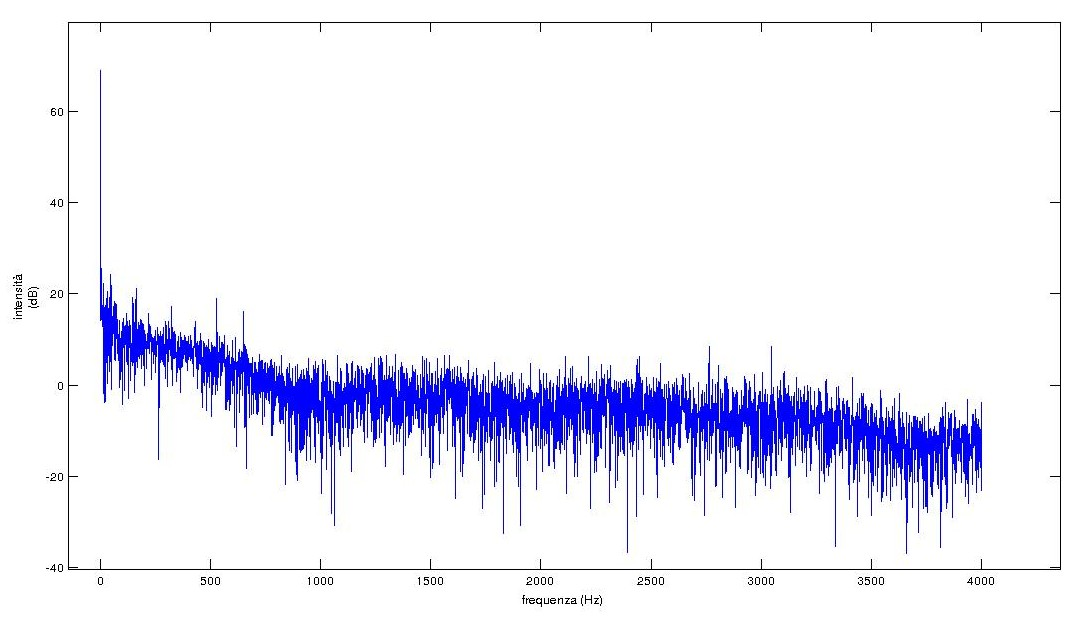
\includegraphics[width=\textwidth*\real{0.9}]{images/ch_02/spettro_rumore.jpg}
	  \end{center} 
	  \caption{\textit{Rumore di registrazione}}  
	  \label{fig:rumore}
	\end{figure}




	\newpage
	\chapter*{I Parametri Fondamentali}\label{cap:parametri}

La seconda operazione da effettuare per la creazione dell'accordatore è la definizione dei parametri di base, cioè la frequenza di campionamento e la durata dell'intervallo temporale.  

Uno dei requisiti fondamentali di un accordatore è la capacità di lavorare in tempo reale. 
In questo contesto, il termine indica che il tempo trascorso tra la ricezione dell'input e la comunicazione dell'output deve essere percepito come istantaneo dall'utente. 
Le operazioni di analisi della frequenza fondamentale della corda, calcolo della distanza tra la frequenza ottenuta e la frequenza di riferimento e comunicazione della risposta, quindi, devono essere effettuate in un intervallo temporale ridotto, il cui limite massimo è stato impostato a 1 secondo dal progettista.
La conseguenza di questo requisito è che la frequenza di campionamento deve essere la più piccola possibile. 
Tenendo conto del teorema del campionamento e supponendo che l'intervallo di frequenze compreso tra 0 e \mbox{4 kHz} contenga informazione sufficiente per rilevare la frequenza fondamentale di ciascuna corda della chitarra, la minima frequenza di campionamento presa in considerazione è di 8 kHz.

Il secondo requisito fondamentale di cui tenere conto nella definizione dei parametri è la precisione dell'analisi della frequenza.
È desiderabile infatti avere un \mbox{JND} almeno pari a quello dell'orecchio umano. 
Questa quantità rappresenta la minima variazione che la frequenza di un suono deve subire affinché il suono risultante venga percepito come distinto dall'originale. 
Il \mbox{JND} è una misura della precisione dell'apparato uditivo umano e dipende dalla frequenza dei suoni.
Per toni complessi che hanno frequenza inferiore ai 500 hz il è di circa 1 hz \todo{riferimento}. 
Dal momento che tutte le frequenze fondamentali delle stringhe della chitarra sono inferiori ai 500 hz, la precisione di 1 hz può essere considerata accettabile.
Fissate la frequenza di campionamento e la risoluzione desiderata, il numero di campioni da analizzare è calcolato dalla seguente formula.

\vspace{0.2cm}
\centerline{\textit{Numero di Campioni = Frequenza di Campionamento / Risoluzione}}
\vspace{0.2cm}

Sostituendo i valori di 1 hz per la risoluzione e di 8 kHz per la frequenza di campionamento, il numero di campioni al secondo risulta essere 8000. 
Questo determina che l'intervallo temporale in cui analizzare nuovi campioni deve essere di un secondo.

I parametri utilizzati per l'accordatore sono i seguenti: frequenza di campionamento di 8 kHz e finestra temporale totale di 1 secondo. 
Nell'intervallo temporale definito, che, come si vedrà nel capitolo dedicato all'interfaccia grafica, è scandito da un timer, non deve essere realizzata solo l'operazione di estrazione dei campioni ma devono essere svolte anche le operazioni di analisi della frequenza del suono, di calcolo della distanza dalla frequenza fondamentale e aggiornamento dell'interfaccia grafica. 
Queste operazioni restringono l'intervallo temporale in cui si estraggono campioni a un intervallo variabile tra 0,65 e 0,89 secondi, con la conseguente riduzione della risoluzione tra i valori 1.56 e 1,12 hz.

Ottenere risoluzioni maggiori a quelle determinate variando solamente frequenza di campionamento e intervallo temporale e rispettando il vincolo di tempo reale definito risulta essere molto difficoltoso. 
A causa del limite di 1 secondo definito dallo sviluppatore, non è possibile estendere la finestra temporale ulteriormente.
Aumentare la frequenza di campionamento, invece, aumenterebbe il numero di campioni da elaborare con il conseguente aumento del tempo di elaborazione e la riduzione dell'intervallo temporale su cui analizzare campioni finendo con il causare una diminuzione di risoluzione.

La soluzione adottata per aumentare la risoluzione è quella dell'interpolazione.
Questa operazione è descritta nella sezione \todo{riferimento}.


	\newpage
	\chapter*{Rilevamento della frequenza fondamentale}\label{cap:rilevamento_frequenza}

L'algoritmo utilizzato per rilevare la frequenza fondamentale è l'algoritmo \emph{Harmonic Product Spectrum}, abbreviato dall'acronimo \emph{HPS}.
Tale metodo sfrutta il fatto che quando viene suonata una nota con uno strumento musicale, l'energia del suono si concentra principalmente nella frequenza fondamentale e nelle sue armoniche, cioè i suoi multipli interi.

L'algoritmo HPS moltiplica lo spettro del segnale con un numero \emph{K-1} di versioni differenti dello spettro.
Le diverse versioni sono ottenute sotto-campionando lo spettro originale con i diversi fattori compresi tra 2 e K.
La formula \ref{formula:hps_prod} descrive la prima parte di questo algoritmo per un generico spettro X( \omega ) e un generico valore \emph{K}.

\begin{equation}\label{formula:hps_prod}
	Y(\omega) = \prod_{i=1}^K \left | X(\omega i) \right |
\end{equation}

Una volta ottenuto il prodotto, la frequenza fondamentale viene calcolata come ascissa del massimo della funzione risultante. 
La formula \ref{formula:hps_max} descrive questo secondo passaggio.

\begin{equation}\label{formula:hps_max}
	Y_{f0} = \max_{\omega_i} Y \left(\omega_i \right )
\end{equation}

 

	\begin{figure}[h]
	  \begin{center} 
	    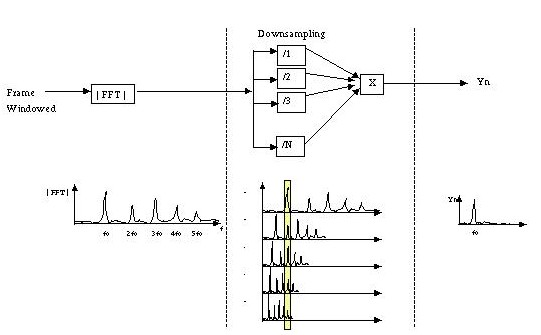
\includegraphics[width=\textwidth*\real{0.9}]{images/ch_04/processo.jpg}
	  \end{center} 
	  \caption{\textit{Rumore di registrazione}}  
	  \label{fig:rumore}
	\end{figure}



	\chapter{Interpolazione}\label{cap:interpolazione}

Come accennato nel capitolo \ref{cap:parametri}, la frequenza di campionamento e il numero di campioni estratti per frame non garantiscono la precisione desiderata.
La soluzione introdotta per aumentare tale precisione è interpolare i valori attorno al massimo trovato.
L'interpolazione utilizzata è di tipo \emph{spline}.
Sono stati interpolati ventuno punti, di cui nove con ascissa inferiore a quella del massimo, il massimo stesso e undici con ascissa superiore al massimo.

	\begin{figure}[h]
	  \begin{center} 
	    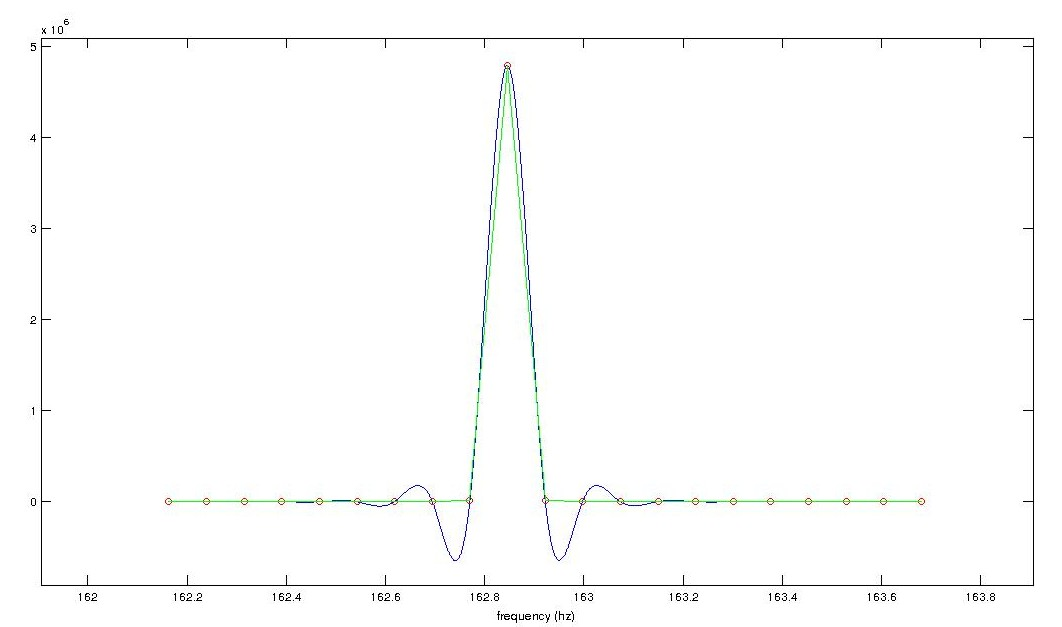
\includegraphics[width=\textwidth*\real{0.9}]{images/ch_05/interpolazione.jpg}
	  \end{center} 
	  \caption{\textit{Interpolazione per migliorare la ricerca del massimo}}  
	  \label{fig:interpolazione}
	\end{figure}

La figura \ref{fig:interpolazione} mostra un esempio di interpolazione. 
I punti evidenziati in rosso, rappresentano il prodotto delle versioni sotto-campionate dello spettro del segnale audio.
La linea verde che li congiunge, rappresenta un'interpolazione lineare.
La linea blu che passa per tutti i punti rappresenta l'interpolazione spline realizzata al fine di trovare il massimo della funzione con una maggiore precisione.

Successivamente all'interpolazione, l'operazione di ricerca del massimo viene effettuata nuovamente e l'ascissa del punto trovato viene utilizzata come frequenza della nota suonata dalla corda della chitarra.

Al fine di eliminare falsi positivi, cioè massimi che possono essere rilevati in momenti in cui non si sta suonando alcuna corda tra quelle della chitarra, è fissata una soglia in ampiezza al di sotto della quale la frequenza del massimo non è ritenuta una frequenza di pitch.
L'algoritmo \mbox{HPS} permette di distinguere nettamente il caso in cui una frequenza fondamentale è presente da quello in cui c'è solamente rumore.
Nel primo caso infatti, la frequenza fondamentale risulta essere molto amplificata, in quanto deriva dal prodotto di 5 massimi locali nelle diverse funzioni scalate della trasformata del segnale originale.
Nel caso del rumore, le diverse frequenze pur moltiplicandosi tra loro non subiscono tale effetto di amplificazione.
La soglia minima al di sopra della quale la frequenza viene considerata fondamentale è fissata a 84 dB.
Si ricorda che il segnale su cui è applicata tale soglia, è il risultato della moltiplicazione di cinque segnali, di conseguenza, in presenza di un pitch, il massimo della funzione è sempre sopra tale soglia.



	\section{Differenza della distanza dalle frequenze di riferimento}\label{cap:distanza}

La frequenza della corda viene confrontata con la frequenza di riferimento desiderata per valutarne la distanza.
La scelta della frequenza di riferimento è descritta nel capitolo \ref{cap:interfaccia}.
La tabella \ref{tab:frequenze_riferimento} contiene per ciascuna corda, il numero di riferimento, la nota prodotta nel caso in cui la corda venga pizzicata e la relativa frequenza di riferimento.

	\begin{table}[h]
	\center
	\begin{tabular}{|l|c|r|}
		\hline
		Corda	& 	Nota    & Frequenza (Hz) \\
		\hline
		1	&	E	&	329.6    \\
		2	&	B	&	246.9    \\
		3	&	G	&	196      \\
		4	&	D	&	146.8    \\
		5	&	A	&	110      \\
		6	&	E	&	82.4     \\		
		\hline
	\end{tabular}
	\caption{\textit{Tabella contenente la frequenza della nota di ciascuna corda della chitarra \cite{giordano2009reasoning}}}
	\label{tab:frequenze_riferimento}
	\end{table}

La distanza tra la frequenza di riferimento e la frequenza del segnale è calcolata con una semplice sottrazione.
In questo caso, l'andamento logaritmico della percezione delle frequenze viene trascurato in quanto la precisione dell'accordatore è stata definita in hertz.

	\chapter{L'interfaccia grafica}\label{cap:interfaccia}

L'interfaccia grafica del programma, oltre a offrire la possibilità di azionare e mettere in pausa l'accordatore, permette di selezionare la modalità con cui definire la frequenza di riferimento, mostra la nota corrispondente a tale frequenza e visualizza la distanza tra la frequenza del suono in input e il valore di riferimento.

È possibile, infatti, indicare esplicitamente la nota da prendere come riferimento oppure lasciar riconoscere all'accordatore tale frequenza in modalità automatica.
Questa seconda opzione risulta comoda quando le corde della chitarra sono leggermente fuori tonalità.
In questo caso, infatti, il software riconosce facilmente la frequenza di riferimento senza la necessità che l'utente debba impostarne il valore manualmente.

	\begin{figure}[h]
	  \begin{center} 
	    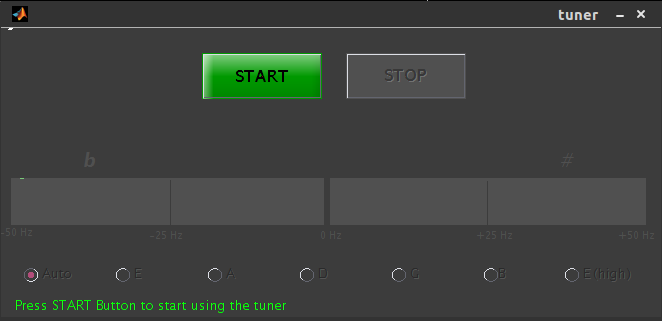
\includegraphics[width=\textwidth*\real{0.8}]{images/ch_07/accordatore_fermo.png}
	  \end{center} 
	  \caption{\textit{Accordatore pronto per essere avviato}}  
	  \label{fig:accordatore_fermo}
	\end{figure}

La figura \ref{fig:accordatore_fermo} mostra la visione che ha l'utente nel momento in cui avvia il programma.
L'accordatore è spento, per azionarlo è necessario premere il bottone \emph{Start}, come suggerisce il messaggio nell'angolo in basso a sinistra della finestra.

Al momento dell'avvio, una serie di operazioni vengono eseguite.
Innanzitutto, viene attivato il timer che regola il funzionamento dell'accordatore.
In secondo luogo, il software avvia la registrazione.
Infine, l'interfaccia grafica viene modificata in modo tale da permettere all'utente di usufruire delle funzionalità del software.

Il timer ha la funzione di chiamare la funzione di tuning una volta al secondo. 
Tale funzione effettua le seguenti operazioni:
\begin{itemize}
	\item fermare il registratore,
	\item estrarre i dati registrati dal buffer del registratore,
	\item riattivare il registratore,
	\item chiamare la procedura di riconoscimento delle frequenza del suono in ingresso,
	\item calcolare la distanza tra frequenza del suono in input e frequenza di riferimento,
	\item aggiornare l'interfaccia grafica con i dati appena calcolati.
\end{itemize}

L'utente ha la possibilità di cambiare la frequenza di riferimento grazie ai bottoni che si trovano appena al di sopra del messaggio di aiuto.

	\begin{figure}[h]
	  \begin{center} 
	    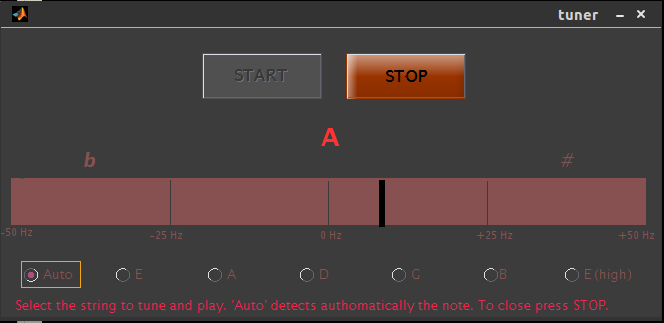
\includegraphics[width=\textwidth*\real{0.8}]{images/ch_07/accordatore_auto.png}
	  \end{center} 
	  \caption{\textit{Accordatore in funzione in modalità automatica}}  
	  \label{fig:accordatore_in_funzione}
	\end{figure}

L'aggiornamento dell'interfaccia consiste nel mostrare la nota di riferimento al di sotto dei bottoni \emph{Start} e \emph{Stop} e nel muovere l'indicatore nero lungo la barra delle frequenze in funzione della distanza misurata tra il suono in input e quello di riferimento. 
In figura \ref{fig:accordatore_in_funzione}, si può vedere l'accordatore, in modalità automatica, mentre fornisce la distanza tra la frequenza della nota in ingresso e la nota di riferimento che, in questo caso, è un LA.




	\newpage
	\chapter{Prestazioni}\label{cap:prestazioni}

Le prestazioni del software sono state testate analizzando le note suonate da una chitarra semiacustica accordata con un accordatore professionale di precisione un cent.
I risultati offerti dal software sviluppato sono conformi alle attese desiderate.
L'unico inconveniente risulta essere una leggera polarizzazione in positivo di circa 0.8 Hz della frequenza identificata per ciascuna nota.
Questo difetto, dovuto alle approssimazioni realizzate nei vari passi dell'algoritmo, può essere facilmente corretto, vista la sua natura sistematica.
La figura \ref{fig:accordatore_in_funzione} mostra questo fenomeno.
Come si può vedere, l'indicatore nero risulta essere leggermente spostato a destra rispetto alla frequenza centrale. 

\begin{figure}[h]
  \begin{center} 
    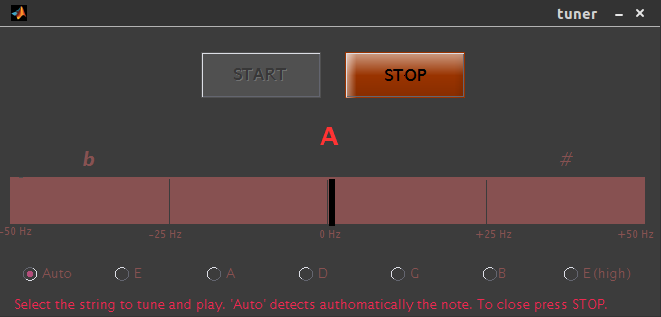
\includegraphics[width=\textwidth*\real{0.8}]{images/ch_08/prestazioni.png}
  \end{center} 
  \caption{\textit{Accordatore in funzione mentre accorda un LA a frequenza 110 Hz. Come si può notare, c'è una leggero spostamento a destra dovuto all'errore sistematico.}}  
  \label{fig:accordatore_in_funzione}
\end{figure}

Un altro fattore che può falsare l'operazione di accordatura è la presenza di disturbi a elevata intensità oppure a bassa intensità ma vicini al microfono. 
In questo caso, infatti, sono presenti delle frequenze aggiuntive che, se comprese nel range [40, 800] Hz, possono essere rilevate come frequenze fondamentali dal software.
La soglia introdotta per distinguere il rumore dalla nota, descritta nella sezione \ref{cap:interpolazione}, risulta essere inutile per questi fenomeni, in quanto, essendo anch'essi dotati di una frequenza fondamentale, presentano un picco ad alta intensità nella funzione prodotto. 
Dal momento che disturbi di questo tipo possono presentarsi a qualsiasi frequenza, risulta impossibile definire un filtro per ridurli. 
Si è quindi deciso di non gestirli.
Anche l'accordatore professionale utilizzato come test, del resto, riconosce le frequenze di questi disturbi.
 
La precisione dell'accordatore professionale, di 1 cent, risulta essere maggiore rispetto a quella del software sviluppato, che nel migliore dei casi, grazie all'interpolazione raggiunge valori di 0,5 Hz.
La relazione logaritmica che lega cent e frequenza, descritta nella formula \ref{formula:cent}, mostra come la precisione raggiunta vari tra i 10 cent a frequenza 82.4 Hz e i 2.62 cent a frequenza di 329.6 Hz.

\begin{equation}\label{formula:cent}
		\Delta_{f_2-f_1} cent = 1200 \log_2 \left( f_2/f_1 \right)
	\end{equation} 

La divisione in cent riflette la modalità di percezione delle frequenze da parte del sistema uditivo umano, di conseguenza, risulta essere una migliore unità di misura per la valutazione della precisione di uno strumento come un accordatore.

Utilizzare una precisione in cent costante richiede l'utilizzo di una scala logaritmica per l'asse delle frequenze.
Ciò significa sostituire la trasformata di fourier discreta, che utilizza un numero di campioni costante tra frequenze successive, con altre trasformate e, di conseguenza, l'implementazione di un altro algoritmo per il rilevamento della frequenza fondamentale delle note.
L'utilizzo di questo tipo di trasformate non è oggetto di questo lavoro.

 


	\newpage
	\chapter{Conclusioni}\label{cap:conclusioni}

In questa relazione viene discussa la creazione di un accordatore digitale per chitarre.
L'operazione più importante da realizzare per raggiungere tale obiettivo è riconoscere la frequenza fondamentale delle note prodotte da una chitarra.
Il risultato di questa operazione è influenzato dal rumore in ingresso e da due parametri fondamentali, frequenza di campionamento e dimensione del frammento temporale.
Questi ultimi due valori dipendono a loro volta dai requisiti temporali e di precisione richiesti.

L'algoritmo utilizzato per riconoscere la frequenza fondamentale delle note musicali si basa sull'algoritmo Harmonic Product Spectrum, che moltiplica diverse versioni scalate dello spettro del segnale e 

Vengono discussi, inoltre, i principali fattori che influenzano l'analisi di tale parametro, cioè il rumore in ingresso, la frequenza di campionamento, la lunghezza del frammento temporale e l'andamento logaritmico della percezione della frequenza. 
Infine viene presentata l'interfaccia grafica, che fornisce una rappresentazione intuitiva per l'utilizzo del programma sviluppato.






	\newpage
	\clearpage


	\pagenumbering{roman}

\end{otherlanguage*}	% da commentare se non si scrive in italiano

%******************************************************************
% Materiale Finale
%******************************************************************
%******************************************************************
%References (two methods in Latex, this (bibTex) with the databe is the best
%******************************************************************
\cleardoublepage
\phantomsection	%gives hyperref something to hold on to when making the link.
\addcontentsline{toc}{chapter}{References}
\bibliographystyle{alpha}				%scelgo come formattare la biblio (abbrv abbrevia i nomi propri. plain non li abbrevia. Ce ne sono un sacco).
\bibliography{beginningEnding/database_references} 	%database dove prendere le info  
\nocite{*}						%stampa TUTTO quello presente nella banca dati, altrimenti solo la roba citata nella tesi

%NB in kile bisogna aggiungere BibTex al QuickBuild per far compilare la bibliografia. Metterlo subito dopo Latex.

\newpage										
\clearpage


\end{document}
